\section{Current Progress}

Before measuring the neutral pion SIDIS cross section, we are preparing the well known inclusive cross section from the same data set.  Doing this adds merit to the results presented in several ways.

\begin{enumerate}
\item Electron identification is validated, because inclusive selection depends only on electrons.
\item Faraday cup charge is validated - Differential cross sections depend on knowing the incoming flux of particles, which in practice is calculated by measuring charge accumulation on a Farday cup.  
\end{enumerate}

\subsection{Inclusive Cross Section Results}

Inclusive inelastic scattering has been measured many times since the early days at SLAC, and is now well understood.  We use a trusted model produced by Cynthia Keppel of JLab based on fits to data to compare with our results.

\begin{figure}
  \centering
  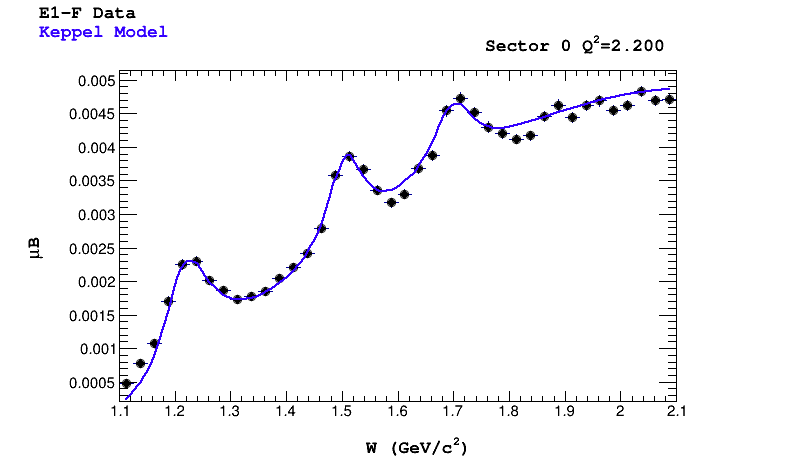
\includegraphics[width=8cm]{image/compareDataModelSector0Slice2.png}
  \caption{Our cross section result compared with Keppel's model.}
  \label{fig:xs}
\end{figure}

\begin{figure}
  \centering
  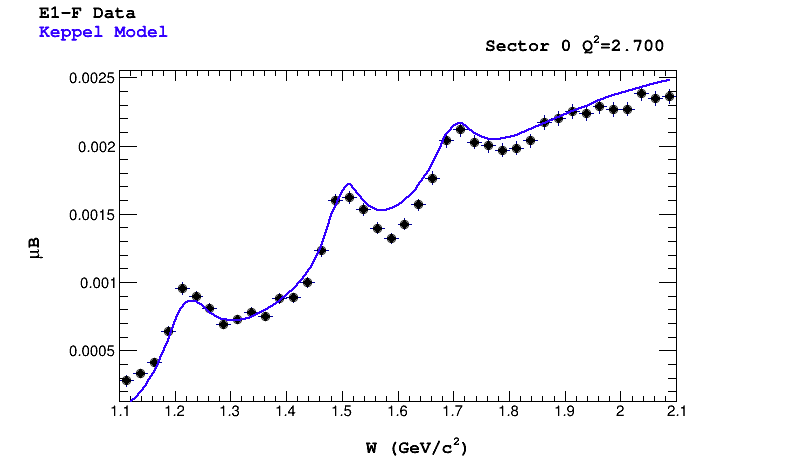
\includegraphics[width=8cm]{image/compareDataModelSector0Slice4.png}
  \caption{Our cross section result compared with Keppel's model.}
\end{figure}

\begin{figure}
  \centering
  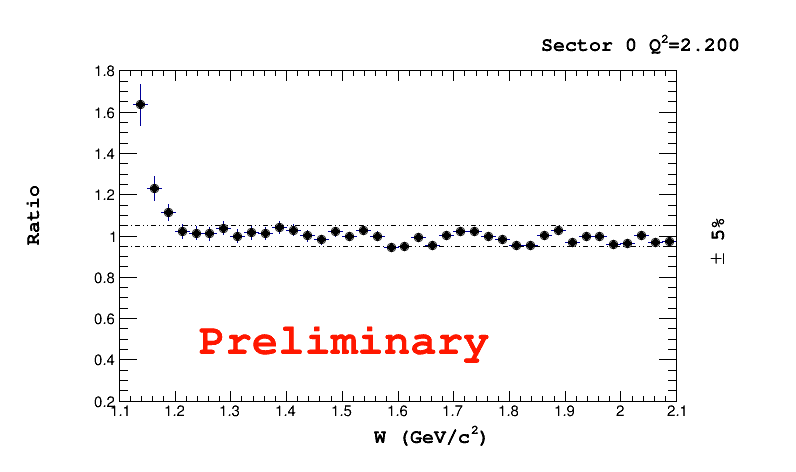
\includegraphics[width=8cm]{image/crossSectionRatioSector0Slice2.png}
  \caption{Ratio of data to Keppel model.}
\end{figure}

\begin{figure}
  \centering
  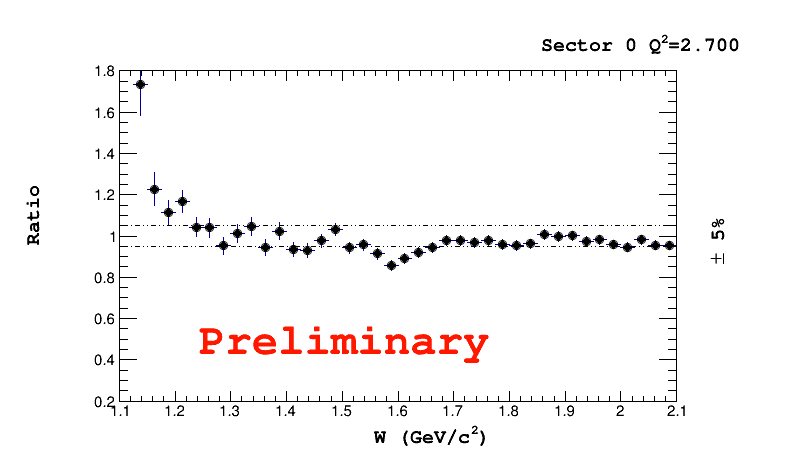
\includegraphics[width=8cm]{image/crossSectionRatioSector0Slice4.png}
  \caption{Ratio of data to Keppel model.}
\end{figure}

